\documentclass[a4paper, 8pt, landscape]{scrartcl}

\usepackage[utf8]{inputenc}
\usepackage[english]{babel}
\usepackage[landscape, margin=1cm, footskip=0.5cm]{geometry}
\usepackage[dvipsnames]{xcolor}
\usepackage{amscd, amsmath, amssymb, blindtext, empheq, enumitem, multicol, parskip, esint}
\usepackage{mathtools}
\usepackage{graphicx}
\usepackage{tikz}
\usepackage{array} %for bigger tabular spacings
\usepackage{pdfpages}
\usepackage{supertabular}
\usepackage{wrapfig}
\usepackage{xcolor}
\usepackage{hyperref}
\usepackage{paralist}
\usepackage[noend,ruled,vlined]{algorithm2e}
\usepackage{caption}
\usepackage{soul}
\usepackage{pifont}% http://ctan.org/pkg/pifont
\newcommand{\cmark}{\ding{51}}%
\newcommand{\xmark}{\ding{55}}%
\usepackage{colortbl}
\usepackage{booktabs}
\usepackage{ccicons}


\newcommand{\highlighty}[1]{%
  \setlength{\fboxsep}{0pt}\colorbox{yellow!100}{\ensuremath{#1}}}

\newcommand{\highlightg}[1]{%
  \setlength{\fboxsep}{0pt}\colorbox{green!100}{\ensuremath{#1}}}

\newcommand{\highlightbg}[1]{%
   \colorbox{green!100}{$\displaystyle #1$}}  

% make document compact
\usepackage[compact]{titlesec}
\titlespacing{\section}{0pt}{*0}{*0}
\titlespacing{\subsection}{0pt}{*0}{*0}
\titlespacing{\subsubsection}{0pt}{*0}{*0}

\parindent 0pt
\pagestyle{plain}
\setlength{\unitlength}{1cm}
\setlist{leftmargin = *}

% Set the color of your style
% Avaiable are: Apricot, Aquamarine, Bittersweet, Black, Blue, blue, BlueGreen, BlueViolet, BrickRed, Brown, BurntOrange, CadetBlue, CarnationPink, Cerulean, CornflowerBlue, Cyan, Dandelion, DarkOrchid, Emerald, ForestGreen, Fuchsia, Goldenrod, Gray, Green, GreenYellow, JungleGreen, Lavender, ... (more at: http://en.wikibooks.org/wiki/LaTeX/Colors)
\def\StyleColor{BurntOrange}

\def\NZ{\mathbb{Z}^{\geq 0}}
\def\N{\mathbb{Z}^{> 0}}
\def\ieq{\overset{!}{=}}
%\DeclareMathOperator{\exp}{exp}
\DeclareMathOperator{\arsinh}{arsinh}
\DeclareMathOperator{\arcosh}{arcosh}
\DeclareMathOperator{\artanh}{artanh}
\DeclareMathOperator{\arcoth}{arcoth}
\DeclareMathOperator{\arccot}{arccot}
\DeclareMathOperator{\limni}{\lim\limits_{n\to\infty}}
\DeclareMathOperator{\limxi}{\lim\limits_{x\to\infty}}
\DeclareMathOperator{\limho}{\lim\limits_{h\to0}}
\DeclareMathOperator{\sumni}{\sum_{n=0}^{\infty}}
\DeclareMathOperator{\partf}{\dfrac{\partial f}{\partial x}}
\DeclareMathOperator{\grad}{grad}
\DeclareMathOperator{\meq}{\stackrel{!}{=}}
\newcommand{\limxai}[1]{\ensuremath{\lim\limits_{x\to #1}}}
\newcommand{\abs}[1]{\ensuremath{\left\vert#1\right\vert}}
\newcommand{\attention}{\raisebox{-1pt}{{\makebox[1.6em][c]{\makebox[0pt][c]{\raisebox{.13em}{\small!}}\makebox[0pt][c]{\color{red}\Large$\bigtriangleup$}}}}}

\newcommand{\partfo}[1]{\ensuremath{\dfrac{\partial f}{\partial #1}}}
\newcommand{\parto}[1]{\ensuremath{\dfrac{\partial }{\partial #1}}}
\newcommand{\partt}[2]{\ensuremath{\dfrac{\partial^2 }{\partial #1\partial #2}}}
\newcommand{\partq}[1]{\ensuremath{\dfrac{\partial^2 }{\partial #1^2}}}

% section color box
\setkomafont{section}{\mysection}
\newcommand{\mysection}[1]{%
    \Large\sf\bf%
    \setlength{\fboxsep}{0cm}%already boxed
    \colorbox{\StyleColor!40}{%
        \begin{minipage}{\linewidth}%
            \vspace*{2pt}%Space before
            #1
            \vspace*{-1pt}%Space after
        \end{minipage}%
    }}

%subsection color box
\setkomafont{subsection}{\mysubsection}
\newcommand{\mysubsection}[1]{%
    \normalsize \sf\bf%
    \setlength{\fboxsep}{0cm}%already boxed
    \colorbox{\StyleColor!20}{%
        \begin{minipage}{\linewidth}%
            \vspace*{2pt}%Space before
             #1
            \vspace*{-1pt}%Space after
        \end{minipage}%
    }}
    
    
% equation box        
\newcommand{\eqbox}[1]{\setlength{\fboxrule}{1mm}\fcolorbox{\StyleColor}{white}{\hspace{0.5em}$\displaystyle#1$\hspace{0.5em}}}


%center equationbox
\newcommand{\ceqbox}[1]{\vspace*{4pt} \begin{center}\eqbox{#1}\end{center}\vspace*{4pt}}
% matrix
\newcommand{\MATR}[1]{ \displaystyle \left( \begin{matrix} #1 \end{matrix} \right)}

%macro for vectors 
%\newcommand{\vect}[1]{\vec{#1}}
\newcommand{\vect}[1]{\boldsymbol{#1}}


\title{Principles of Distributed Computing}
\author{Yannick Merkli \\ymerkli@student.ethz.ch}
\date{\today}


\begin{document}

%\setcounter{secnumdepth}{0} %no enumeration of sections
\begin{multicols*}{3}
	
\section*{Disclaimer}

This document is an exam summary that follows the script of the \textit{Principles of Distributed Computing} lecture  at ETH Zurich. The contribution to this is a short summary that includes the most important formulas, algorithms and proof ideas. This summary was created during the spring semester 2020. Due to updates to the syllabus content, some material may no longer be relevant for future versions of the lecture. This work is published as CC BY-NC-SA.

\begin{center}
	\ccbyncsa
\end{center}

I do not guarantee correctness or completeness, nor is this document endorsed by the lecturers. Feel free to point out any erratas. For the full \LaTeX \ source code, consider \texttt{\href{https://github.com/ymerkli/eth-summaries}{github.com/ymerkli/eth-summaries}}.
	
\newpage	

\maketitle 
\section*{General}
\begin{compactitem}
	\item \textbf{Synchronous Algorithms} perform in rounds consisting of:
	(1) Send msgs to neighbors (2) Receive msgs from neighbors (3) do some local computation.
	\item \textbf{Asynchronous Algorithms} are event driven: Upon... do...;	No global clock available. Nodes have to wake up!
	\item \textbf{Anonymous}: nodes can’t distinguish each other, no unique IDs
	Uniform: nodes don’t know n
	\item \textbf{Clean}: nodes don’t know the topology
	\item \textbf{Distance of two nodes}: the amount of hops on the shortest path between them (adjacent nodes have distance 1)
	\item \textbf{Radius of a node}: max distance from node to any other node
	\item \textbf{Radius of graph}: min radius of any node
	\item \textbf{Diameter of graph}: max distance between two arbitrary nodes.
	\item $R \leq D \leq 2R$
	\item For tree: depth of a node is distance from root. Height is maximal distance to any leaf. Depth(root) = 0; Height(root) = depth(tree); Height(leaf) = 0
	\item \textbf{Symmetric graph}: neighborhoods of all nodes “look” the same
\end{compactitem}
\subsection*{Common variables}
n = \# of nodes; m = \# of edges; $\Delta$ = maximum degree of any vertex; D = Diameter; R = Radius; (M)ST = (Minimum) Spanning Tree;

\subsection*{Functions}

Log-Star: $\forall x \leq 2: \log^*x := 1; \forall x > 2: \log^*x := 1 + \log^*(\log x)$


\section{Vertex Coloring}

\textbf{Vertex Coloring}: Given an undirected graph $G=(V,E)$, assign a color $c_v$ to node $v \in V$ s.t. no two adjacent nodes $v,w \in V$ have the same color: $c_v \neq c_w$.

\textbf{Chromatic number $\chi(G)$}: On an undirected graph $G=(V,E)$, the chromatic number $\chi(G)$ is the minimum number of colors to solve vertex coloring.

\subsection{Basic Coloring Algorithms}

\textbf{Greedy Sequential}: Simple non-distributed ("centralized") vertex coloring algorithm. Iterates over nodes and assigns minimal free color in $\{1,...,\Delta+1\}$.

\columnbreak

\textbf{Reduce}: First, all nodes exchange Ids among neighbor nodes. Then in each round, the uncolored node with max. Id in its neighborhood chooses the smallest admissible color and informs its neighbors about its choice. \textbf{Time:} $\mathcal{O}(n)$, \textbf{Colors}: $\mathcal{O}(\Delta+1)$, \textbf{Msgs:} $\mathcal{O}(2n\Delta)$.

\subsection{Coloring Rooted Trees}

\textbf{Lemma 1.13}: $\chi(Tree) \leq 2$.

\textbf{Slow tree coloring:} Assumes directed tree (each node knows its parent). Color the root $r$ $c_r = 0$, root sends 0 to children. Every node $v$ when receiving color $c_p$ from parent, colors itself to $c_v = 1 - c_p$ and sends $c_v$ to its children. \textbf{Time}: $\mathcal{O}(n)$, \textbf{Colors}: 2.

\textbf{6-Color:} Initially, each node $v$ has color $c_v$ of $\log n$ bits. Each node then sends $c_v$ to all children, receives $c_p$ from parent and finds the index $i$ of the rightmost bit $b$ where $c_v$ and $c_p$ differ. $v$ recolors itself to $c_v = 2i + b$. This is done until $c_v \in \{0,...,5\}$. \textbf{Time}: $\mathcal{O}(\log^* n)$, \textbf{Colors}: 6.

\textbf{Shift Down:} Node recolors itself to parent's color. Root chooses new (different) color from $\{0,1,2\}$. This makes all siblings monochromatic. \textbf{Time:} $\mathcal{O}(1)$. \textbf{Color:} 3.

\textbf{Six-2-Three:} Each node $v$ concurrently executes the following:\\
{
\setlength{\interspacetitleruled}{0pt}%
\setlength{\algotitleheightrule}{0pt}%
\begin{algorithm}[H]
	\SetAlgoLined
	\For{$x = 5,4,3$}{
		Perform Shift Down\;
		\If{$c_v = x$}{
			choose smallest admissible new color $c_v \in \{0,1,2\}$
		}
	}
\end{algorithm}
}

\textbf{Theorem 1.23:} 6-Color together with Six-2-Three colors a tree in \textbf{Time}: $\mathcal{O}(\log^* n)$, \textbf{Colors}: 3.

\section{Tree Algorithms}

\textbf{Definition 2.5} (Clean): A graph (network) is \textit{clean} if the nodes do not know the topology of the graph.

\textbf{Definition 2.8} (\hl{Asynchronous Time Complexity}): For asynchronous algorithms the time complexity is the number of time units from the
start of the execution to its completion in the worst case. For each message, we have \hl{\textbf{msg\_transit\_time } $\leq$ \textbf{ 1 time unit }}.

\textbf{Broadcast}: send message from single node, the “source”, to all other nodes in the topology. Flooding is a simple broadcast algorithm. Broadcast lower bound $\mathcal{O}(n)$.

\textbf{Convergecast}: opposite of broadcast: All nodes send information to one single node. Echo is a simple convergecast algorithm. Combine Echo \& Flooding to collect information about entire graph.

\textbf{Flooding}: The source node sends the broadcast to all neighbors, all other nodes forward the broadcast to all their neighbors, replicas are dropped. \textbf{Time} (sync/async): $\mathcal{O}(radius(src)) = \mathcal{O}(n)$.

\textbf{Echo}: All leaves send the Echo msg to their parents. Parent nodes wait for all children’s msgs and then send the merged msg to their parent. Msgs are merged according to the type of data collected (add, min, max, avg, concatenation, ...). \textbf{Time} (sync/async): $\mathcal{O}(n)$.

\columnbreak

\textbf{Flooding/Echo}: Combine Flooding and echo.

\vspace*{-2mm}
\begin{center}
\renewcommand{\arraystretch}{1.1}
\begin{tabular}{@{}ccc@{}}
	\hline 
	& async & sync \\ 
	\hline 
	Time & $\mathcal{O}(n)$ & $\mathcal{O}(D) = \mathcal{O}(n)$ \\ 
	Msg & $\mathcal{O}(m+n)$ & $\mathcal{O}(m+n)$ \\ 
	\hline 
\end{tabular} 
\end{center}

\subsection{Applications of flooding/echo}

\textbf{Create a spanning tree with flooding}: If every node considers the neighbor from which the broadcast came as parent, flooding creates a spanning tree with the source as root. If the flooding is performed synchronously the resulting spanning tree is breadth-first. In asynchronous networks a breadth-first tree can be created using the Dijkstra BFS or Bellman Ford BFS algorithms.

\textbf{Count nodes in network with flooding/echo}: In the Echo part every node sends the sum of children’s messages +1 to their parent.

\textbf{Assigning unique IDs}: First perform flooding / echo to count the number of nodes, every node stores the sizes of their children. In a second flooding the available ID range is split among the children according to their sizes.

\subsection{BFS Tree Construction}

Flooding constructs a BFS \textit{in the sync setting}. In the async setting, we can use Dijkstra or Bellman Ford.

\textbf{Dijkstra BFS}: Always adds the "closest" node to the existing part of the BFS tree, developing the BFS tree layer by layer. The root starts phase p by flooding "start p" in T. Leafs that receive "start p" send "join p+1" to quiete neighbors. If a node not yet in T receives "join p+1", it replies ACK, else replies "NACK". Leaves that sent join msgs collect ACKs/NACKs and echo back to root.\\
\textbf{Time:} $\mathcal{O}(D^2)$, \textbf{Message}: $\mathcal{O}(m+nD)$.

\textbf{Bellman-Ford BFS}: All nodes keep the distance to the root accurate. Initially, root has $d_{root} = 0$ and all other nodes have $d_v = \infty$. Root starts by sending "1" to neighbors. If a node $v$ receives a message with $y < d_v$, it updates $d_v := y$ and sends "y+1" to all neighbors. \textbf{Time:} $\mathcal{O}(D)$, \textbf{Message}: $\mathcal{O}(nm)$.

\textbf{Optimized BFS construction:} optimizes Dijkstra and Bellman-Ford. \textbf{Time:} $\mathcal{O}(D\log^3 n)$, \textbf{Message}: $\mathcal{O}(m + n\log^3 n)$.

\subsection{MST Construction}

\textbf{Definition 2.15} (MST): The MST is a spanning tree on a weighted graph $G = (V,E,\omega)$ minimizing the weight of the tree edges $\omega(T)$.

\textbf{Blue edges}: The minimum weight outgoing edge $e = (u,v) = b(T')$ of a subgraph $T' \subseteq T$, with $u \in T', v \notin T'$, is the so-called blue edge.

\textbf{Lemma 2.17}: Let $T$ be the MST of G and let $T'$ be a fragment of $T$. Then the blue edge of $T'$ is in $T$.

\textbf{GHS algorithm}: computes a MST on weighted undirected graph without needing an initial leader.  Initially all nodes are root of their own fragment. Fragments have a root and are repeatedly merged along blue edges. In every round the blue edge is located and the root is moved to the blue edge (inverting hierarchy on the path). All blue edges merge the corresponding fragments. Inside a fragment we use flooding/echo to spread information.\\ \textbf{Time:} $\mathcal{O}(n\log n)$, \textbf{Message}: $\mathcal{O}(m\log n)$.

\newpage

\section{Distributed Graph Coloring}

\textbf{Cover free families}: Given a ground set $\{1,2,...,k'\}$, a family of sets $S_1, S_2, ..., S_k \subseteq \{1,2,...,k'\}$ is called a $\Delta$-cover free family if for each set of $\Delta + 1$ indices $i_0, i_1, ..., i_{\Delta} \in \{1,2,...,k\}$, we have $S_{i_0} \backslash (\bigcup_{j=1}^{\Delta} S_j) \neq \emptyset$. That is, if no set in the family is a subset of the union of $\Delta$ other sets.

\textbf{Lemma 1.18}: For any $k$ and $\Delta$, there exists a $\Delta$-cover free family of size $k$ on a ground set of size $k' = \mathcal{O}(\Delta^2 \log k)$.

\textbf{Lemma 1.19}: For any $k$ and $\Delta \geq k^{1/3}$, there exists a $\Delta$-cover free family of size $k$ on a ground set of size $k' = \mathcal{O}(\Delta^2)$.

\textbf{Lemma 1.20}: Given a $k$-coloring $\phi_{old}$ of a graph with max degree $\Delta$, in a single round, we can compute a $k'$-coloring $\phi_{new}$, for $k' = \mathcal{O}(\Delta^2 \log k)$. Further, if $k \leq \Delta^3$, then the bound can be improved to $k' = \mathcal{O}(\Delta^2)$.

\textbf{Linial's Coloring Algorithm}: Deterministic distributed algorithm in the LOCAL model that colors any n-node graph $G$ with max degree $\Delta$ using \hl{$\mathcal{O}(\Delta^2 \log \Delta)$ (or $\mathcal{O}(\Delta^2)$) colors}, in \hl{$\mathcal{O}(\log^* n)$ rounds}. The algorithm follows from repeated applications of Lemma 1.20. 

\subsection{Kuhn-Wattenhofer Coloring Algorithm}

\textbf{Basic idea}: Use Linial to get a $\mathcal{O}(\Delta^2 \log \Delta)$-coloring in $\mathcal{O}(\log^* n)$ rounds. Then reduce colors in $\mathcal{O}(\Delta \log \Delta)$ rounds.

\textbf{One-by-one color reduction}: Given a $k$-coloring $\phi_{old}$ of a graph with max degree $\Delta$ where $k \geq \Delta + 2$, in a single round, we can compute a $(k-1)$-coloring $\phi_{new}$. This can be done by letting all nodes $v$ with $\phi_{old}(v) = k$ choose a new color in $\{1, ..., \Delta+1\}$.

\textbf{Theorem 1.22}: Combining Linial with repeated one-by-one color reduction gives a deterministic coloring algorithm in the LOCAL model that colors any $n$-node graph with max degree $\Delta$ using $\Delta+1$ colors in $\mathcal{O}(\Delta^2 + \log^* n)$ rounds.

\textbf{Parallelized color reduction}: Given a $k$-coloring $\phi_{old}$ of a graph with max degree $\Delta$ where $k \geq \Delta+2$, we can compute a $(\Delta+1)$-coloring in $\mathcal{O}(\Delta \log(\frac{k}{\Delta + 1}))$ rounds. If $k \leq 2\Delta + 1$, this follows directly. Else, we can bucketize colors into $\lfloor \frac{k}{2\Delta + 2} \rfloor$ and perform one-by-one color reduction in all buckets in parallel.

\textbf{Theorem 1.23 (Kuhn-Wattenhofer Coloring Algorithm)}:\\
Deterministic distributed algorithm in the LOCAL model that colors any n-node graph G with max degree $\Delta$ using \hl{$\Delta+1$ colors}, in \hl{$\mathcal{O}(\Delta \log \Delta + \log^* n)$ rounds}. The algorithm uses Linial to get a $\mathcal{O}(\Delta^2)$-coloring in $\mathcal{O}(\log^* n)$ rounds and then uses parallelized color reduction in $\mathcal{O}(\Delta \log \Delta)$ rounds.

\textbf{Theorem 1.25} (Kuhn's Algorithm via Defective Coloring)\\
There is a deterministic distributed algorithm in the LOCAL model that colors any $n$-node graph $G$ with maximum degree $\Delta$ using $\Delta+1$ colors, in $\mathcal{O}(\Delta + \log^* n)$ rounds.

Yet another $\mathcal{O}(\Delta \log \Delta + \log^* n)$ $(\Delta+1)$-coloring algorithm: see exercise 3.3 (disjoin nodes by their ID bit-by-bit).

\columnbreak

\section{\large{Lower Bounds on Distributed Graph Coloring}}

Locality as a limitation in distributed systems.\\
Basic intuition: \hl{2-coloring any n-path graph requires $\mathcal{O}(n)$ rounds.}

\textbf{Theorem 1.7}: Any deterministic algorithm for 3-coloring n-node directed paths needs at least $\frac{\log^* n}{2} - 2$ rounds.

\textbf{Definition 1.8:} We say $B$ is a k-ary q-coloring if for any set of identifiers $1 \leq a_1 < a_2 < ... < a_k < a_{k+1} \leq n$, we have the following properties:
\vspace*{-2mm}
\begin{compactenum}
\item $B(a_1, a_2, ..., a_k) \in \{1,2,...,q\}$
\item $B(a_1, a_2, ..., a_k) \neq B(a_2, ..., a_{k+1})$
\end{compactenum}

\textbf{Lemma 1.10:} There is no 1-ary $q$-coloring with $q < n$.

\textbf{Lemma 1.11:} If there is a k-ary $q$-coloring B, then there exists a (k-1)-ary $2^q$-coloring B'.


\subsection{Coloring Unrooted Trees}

\textbf{Theorem 1.12}: Any (deterministic) distributed algorithm $\mathcal{A}$ that colors n-node trees with max degree $\Delta$ using less than $\mathcal{O}(\frac{\Delta}{\log \Delta})$ colors has round complexity at least $\Omega(\log_{\Delta}n)$.

\textbf{Theorem 1.14}: There is a deterministic distributed algorithm that computes a \hl{3-coloring of any n-node tree in $\mathcal{O}(\log n)$ rounds.}

\textbf{Algorithm for coloring unrooted Trees:}\\
(1) Perform an \hl{iterated peeling process} on given tree $T=(V,E)$. First, let $T_1 = T$ and $L_1$ the set of all vertices in $T_1$ whose degree in $T_1$ is at most 2. Then, let $T_2 = T_1 \backslash L_1$. Iterate this process. Generally, each $T_{i+1}$ is defined as $T_{i+1} = T_i \ L_i$ and $L_{i+1}$ consists of all vertices in $T_{i+1}$ that have degree at most 2 in $T_{i+1}$. \textbf{Time:} $\mathcal{O}(\log n)$.\\
(2) Color each subgraph $T[L_i]$ independently using 3 colors in $\mathcal{O}(\log^* n)$ rounds, using Theorem 1.23. Then use the colors of the graphs $T[L_i]$ as a schedule color for computing the final output coloring of the vertices. \textbf{Time:} $\mathcal{O}(\log^* n)$

Overall: \textbf{Time} $\mathcal{O}(\log n)$



\section{Maximal Independent Set (MIS)}

\textbf{Independent set}: A set $S$ is an independent set if no two vertices $u, v \in S$ are adjacent.

\textbf{Maximal independent set}: A set $S$ is a maximal independent set if we cannot add any node $v \notin S$ to the set $S$ without violating the independent set condition.

\textbf{Dominating set}: subset of nodes such that every node is either in the set or adjacent to a node in the set. The minimum dominating set is the smallest DS that can be found. Any MIS is a DS.

\textbf{Slow MIS}: a node joins the MIS if all neighbors with higher ID have decided not to join the MIS. \textbf{Time:} $\mathcal{O}(n)$, \textbf{Msg:} $\mathcal{O}(m)$.

\textbf{Lemma 1.50}: Given a LOCAL algorithm $\mathcal{A}$ that computes a MIS on any N-node graph G in $T(N)$ rounds, there is a LOCAL algorithm $\mathcal{B}$ that computes a $\Delta+1$ coloring of any n-node graph with max degree $\Delta$ in $T(n(\Delta+1))$ rounds.
\textbf{Proof}: Run MIS algorithm $\mathcal{A}$ on graph $H = G \times K_{\Delta+1}$. $H$ contains $\Delta+1$ copies of $G$ where all $\Delta+1$ copies of a node $v$ are in a clique (i.e. they are all connected). For node $v$ copy, check which copy is in the MIS, that copy Id is the node color.

\subsection{Luby's MIS algorithm}

\textbf{Luby's algorithm}: The algorithm is made of iterations, each of which has two rounds:

\begin{compactenum}
\item Each node $v$ picks a real number $r_v \in [0.1]$ and sends it to all neighbors. A node $v$ joins MIS set $S$ iff $r_v$ is a strict local maximum, i.e. $r_v > r_u, \forall u \in N(v)$.

\item If a node $v$ joined $S$, it informs all its neighbors and all neighbors are removed from the problem.
\end{compactenum}

\textbf{Theorem 1.51:} \hl{Luby's algorithm finds a MIS in $\mathcal{O}(\log n)$ rounds with high probability.}\\
The basic idea of the proof is as follows: Event $X_{w\rightarrow e}$: node $w \in N(u)$ single-handedly kills edge $e=(u,w)$ if $w$ has max value $r_w$ among $N(w) \cup N(u)$; $P(X_{w\rightarrow e}) \geq \frac{1}{d(w)+d(w)}$. Analyzing the number of edges from iteration $i$ to $i+1$ shows that the number of edges drops by at least $1/2$ w.h.p. The $\mathcal{O}(\log n)$ round follows directly.


\section{Network Decomposition}

\textbf{LOCAL model}: undirected n-node graph $G=(V,E)$, one 'computer' on each node, nodes have IDs in $\{1,2,..., poly(n)\}$, nodes pass \hl{unbounded msgs} in rounds.

\textbf{Basic intuition}: Most problems can be solved easily by collecting graph topology in one node and solving it locally (using some local algorithm). Collecting the graph topology only works in small diameter networks ($poly(\log n)$). Using network decomposition, we can cluster graph into small diameter subsets.

\textbf{(C,D) Network Decomposition}: A (C,D) network decomposition partitions nodes of a graph $G=(V,E)$ into clusters of diameter at most $D$, where each cluster is assigned a color in $\{1,...,C\}$ such that adjacent clusters have different colors.

\begin{compactitem}
\item Strong diameter: Diameter $D$ of cluster is measured on cluster-induced subgraph, i.e. paths only along edges that have both endpoints in the cluster.
\item Weak diameter: Diameter $D$ of cluster is measured on the base graph $G$.
\end{compactitem}

\subsection{Rozhon Ghaffari Network Decomposition}

\textbf{Theorem [Rozhon, Ghaffari 2020]}: A deterministic algorithm that constructs a \hl{$(C,D)$ network decomposition with $C=\mathcal{O}(\log n)$ colors and $D=\mathcal{O}(\log n)$ cluster diameter in $poly(\log n)$ rounds}. In this lecture, we look at a slightly weaker version with $C=\mathcal{O}(\log n)$, weak-diameter $D=\mathcal{O}(\log^3 n)$ in $\mathcal{O}(\log^7 n)$ rounds.

This algorithm leads to $poly(\log n)$ rounds deterministic algorithms for many central problems such as MIS, $\Delta+1$ coloring, ...

\textbf{Algorithm} (one run gives one cluster color): Each node has $\mathcal{O}(\log n)$-bit Id. We have $\mathcal{O}(\log n)$ phases, in each of which we treat one bit of the Id. In phase $i$, nodes are grouped by their $i$-th Id bit, where nodes with $i$-bit 1 are {\color{blue}blue} and nodes with $i$-bit 0 are {\color{red}red}. All nodes with equal Id are in a cluster. Red nodes are selfish and try to join a blue cluster by sending a request. Blue clusters accept all red nodes that sent requests in one step if it means multiplicative increase by a factor of $1 + 1/\mathcal{O}(\log n)$. Blue clusters know \#requests through flooding (clusters have small diameter $\mathcal{O}(\log^3 n)$).\\
If the increase is too small, the blue cluster denies all red nodes that sent requests and those red nodes are dead (grey) for that phase. A red node that joined a blue cluster changes its whole Id to the Id of the cluster (the Id of the original cluster vertex). Note: when a blue cluster stops growing, it never grows again during the current phase.\\
Claim: in $\mathcal{O}(\log^2 n)$ growth steps, all blue clusters stop growing. Reason: You can only grow at rate $\geq 1 + 1/\mathcal{O}(\log n)$ $\mathcal{O}(\log^2 n)$ many times. Cluster radius increases by $\mathcal{O}(1)$ per growth step. Since we have $\mathcal{O}(\log^2 n)$ growth steps, each cluster's weak diameter grows additively by $\mathcal{O}(\log^2 n)$ per phase.

After $i$-th phase, there is no edge between two clusters with different $i$-th bit in their label, i.e. connected components agree on the $i$-th bit. After $\mathcal{O}(\log n)$ phases, all remaining clusters are non-adjacent.

In each of the $\mathcal{O}(\log n)$ phases, we deleted $\mathcal{O}(1/\log n)$ fraction of vertices (due to small cluster growth), thus over all phases at most $1/2$ of vertices are deleted. Thus, we always color at least $1/2$ of vertices per phase.

Analysis: $\mathcal{O}(\log n)$ phases, $\mathcal{O}(\log^2 n)$ additive diameter growth per phase, thus $D=\mathcal{O}(\log^3 n)$. One phase has $\mathcal{O}(\log^2 n)$ growth steps. Deciding whether to grow a cluster in a growth step requires Convergecasting, which has $\mathcal{O}(D) = \mathcal{O}(\log^3 n)$. One such full run of the algorithm gives one color, to get the full network decomposition, the algorithm needs to be run $\mathcal{O}(\log n)$ many times (since in each run, at least $1/2$ of nodes are clustered).

$Time_{tot}$: $\mathcal{O}(\log n) * \mathcal{O}(\log n) * \mathcal{O}(\log^2 n) * \mathcal{O}(\log^3 n) = \mathcal{O}(\log^7 n)$

\subsection{Randomized Construction}

\textbf{Theorem 1.31:} There is a randomized LOCAL algorithm that computes a $(C,D)$ weak-diameter network decomposition of any $n$-node graph $G$, for \hl{$C = \mathcal{O}(\log n)$ and $D = \mathcal{O}(\log n)$, in $\mathcal{O}(\log^2 n)$ rounds, with high probability.} The round complexity of this construction \hl{can be improved to $\mathcal{O}(\log n)$ rounds.}

\subsection{Applications}

\textbf{MIS}: Calculate (C,D) network decomposition. Use cluster color as scheduling color. Use $\mathcal{O}(\log n)$ phases, in phase $i$, all clusters of color $i$ compute a MIS on their cluster using a local bruteforce approach (collect topology at leader node). After one round, node inform neighbors if it joined MIS. Since equal color clusters are mutually non-adjacent, two adjacent nodes in different clusters are never added to the MIS in the same round. \textbf{Time:} $\mathcal{O}(CD)$.

\textbf{Triangle-free subset}: Calculate (C,D) network decomposition. Use cluster color as scheduling color. Use C phases, in phase $i$, all clusters of color $i$ compute a triangle-free subset on their cluster and inform neighbors. \textbf{Time:} $\mathcal{O}(CD)$.


\section{Shared Objects}

There is a common resource in a network which different nodes want to access from time to time.

\textbf{Algorithm 7.1} (Centralized solution): root node $r$ holds resource and processes requests atomically. This is inefficient.

\textbf{Algorithm 7.2} (Home-based solution): A resource has a home base. A node $v$ that requested the resource receives the object. Following requests are routed through the homebase to $v$. This suffers from the triangular routing problem.

\subsection{Arrow and Friends}

\begin{center}
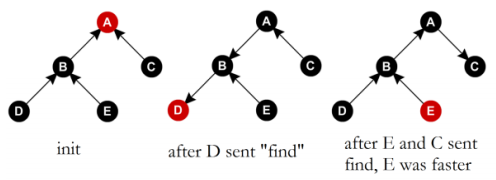
\includegraphics[width=0.7\columnwidth]{source/arrow}
\end{center}


\textbf{Arrow Algorithm}: Runs on a precomputed spanning tree, object stored at root. Each node has a parent pointer, i.e. we have a directed tree. If a node wants to access the object, it gets the object with a find request. The "find" follows the edge pointers and inverts each edge direction once it passed the edge.  All parent/child relations are thus inverted. Object is sent using routing (doesn’t care about arrows). The node that sent the "find" becomes the new root.

\textbf{Theorem 7.4}: In an asynchronous and concurrent setting, a “find” operation terminates with message and \hl{time complexity $\mathcal{O}(D)$,} where $D$ is the diameter of the spanning tree.

\textbf{Theorem 7.6}: Arrow is at most $\log n$ worse than the best possible tour (optimal vs. greedy traveling salesman problem).

\textbf{Read/write caching} (Adaption of arrow to increase read speed):\\
Use caching. The find operation is replaced by a write and a read operation. A read operation does not need to move the object to the initiator of the read, he just has to find a close node that has a cache of the object. On the way back a copy of the object is cached in every hop and all cache bits on the path are set. If a node wants to write it first finds a node with a copy. It deletes the copy and follows the cache bits to delete all other copies (each node has cache bits for each edge). On the way back, it redirects parent pointers towards the new root if necessary. The node that initiated the write becomes new root.


\subsection{Ivy and Friends}

\textbf{NOTE:} Ivy assumes a complete graph, i.e. each node is connected to each node.

\begin{center}
	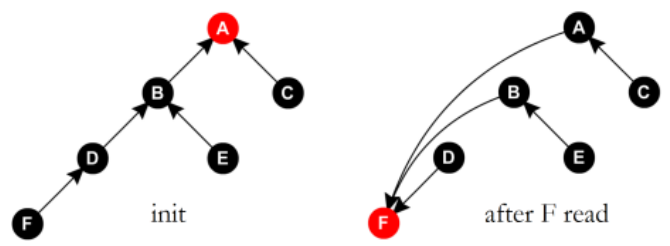
\includegraphics[width=0.5\columnwidth]{source/ivy}
\end{center}

\textbf{Ivy Algorithm}: Runs on a precomputed spanning tree, object stored at root. Each node has a parent pointer. A node $u$ that wants to access the object sends "find by u". The msg follows the edge directions and on the way all parent pointers of nodes on the path visited during the "find" are redirected to $u$ (the new root).

\textbf{Theorem 7.12}: If the initial tree is a star, a find request of the Ivy algorithm needs \hl{at most $\log n$ steps on average}.


\section{Distributed Sorting}

\textbf{Definition 8.1} (Sorting): We choose a graph with $n$ nodes $v_1, ..., v_n$. Initially each node stores a value. After applying a sorting algorithm, node $v_k$ stores the
k-th smallest value.

\textbf{Definition 8.2} (Node Contention): In each step of a synchronous algorithm, \hl{each node can only send and receive O(1) messages containing O(1) values}, no matter how many neighbors the node has.


\subsection{Array \& Mesh}

\textbf{Odd/ Even Sort} (works on array (x – x – x), nodes need to know if they are odd or even): Alternatingly, all odd and even nodes are compared to their right neighbors. The values are switched if necessary. \textbf{Time}: $\mathcal{O}(n)$

\textbf{Lemma 8.4 (0-1 Sorting Lemma)}: If an oblivious comparison-exchange algorithm sorts all inputs of 0’s and 1’s, then it sorts arbitrary inputs.

\textbf{Shearsort}: Sorts a $n = m \times m$ grid in a snake-like order. Sorting proceeds in phases: Odd phases (1,3,..) sort rows, even phases (2,4,..) sort columns. Columns: small values move up. Odd [even] rows: small values move left [right]. \textbf{Time}: $\mathcal{O}(\sqrt{n}(\log(n) + 1))$


\subsection{Sorting Networks}

\begin{minipage}{\columnwidth}
	\centering
	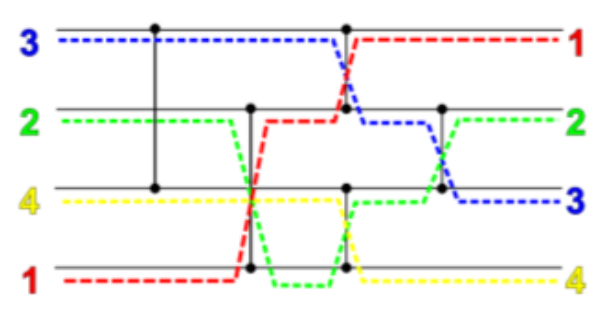
\includegraphics[width=0.45\columnwidth]{source/sortingnetwork}
	\vspace*{-2mm}
	\captionof*{figure}{Example sorting network}
\end{minipage}%

\textbf{Definition 8.8} (Sorting Networks). A comparator is a device with two inputs $x, y$ and two outputs $x_0, y_0$ such that $x_0 = min(x, y)$ and $y_0 = max(x, y)$. A sorting network consists of a set of wires that connect comparators according to some schema.\\
\textbf{Width} = number of input wires (= number of output wires).

A sorting network is an oblivious comparison-exchange network, thus \hl{apply the 0-1 sorting Lemma}.

\textbf{Definition 8.10} (Depth): The depth of an input wire is 0. The depth of a comparator is the max. depth of its input wires +1. The depth of an output wire of a comparator is the depth of the comparator. The depth of a sorting network is the max. depth. 

\textbf{Definition 8.11} (Bitonic Sequence): A bitonic sequence is a sequence of numbers that first monotonically increases, and then monotonically decreases, or vice versa. Example: $[1,4,6,3,2]$, $[0,0,1,1,0,0,0]$. There are $(n+1)n/2 + 1$ possible 0-1 bitonic sequences.


\textbf{Half Cleaner}: A half cleaner is a comparison network of depth 1. If we input a bitonic sequence to a half cleaner, one half of the output will be clean (all-0 or all-1), the other half will be a bitonic sequence.\\
Width = powers of 2. Depth = 1.

\textbf{Bitonic Sequence Sorter (BSS)}: A BSS of width $n = 2^k$ sorts bitonic sequences. It has depth $\mathcal{O}(\log n)$. A BSS of width 1 is empty.

\vspace*{-1mm}
\begin{minipage}{0.5\columnwidth}
	\centering
	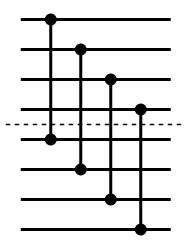
\includegraphics[width=0.47\columnwidth]{source/halfcleaner}
	\captionof*{figure}{Half cleaner of width 8}
\end{minipage}%
\begin{minipage}{0.5\columnwidth}
	\centering
	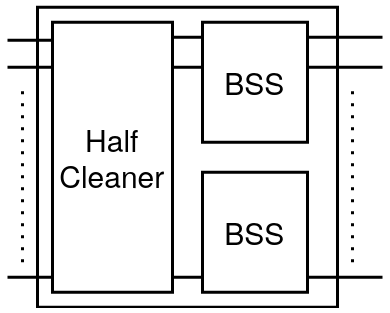
\includegraphics[width=0.75\columnwidth]{source/bss}
	\captionof*{figure}{Bitonic Sequence Sorter}
\end{minipage}
\vspace*{-1mm}

\textbf{Merger}: A merger takes two sorted sequences as input and converts them into two bitonic sequences. Depth = 1.

\textbf{Merging Network}: A merging network of width $n$ is a merger followed by two BSS of width $n/2$. A merging network of width $n$ merges two sorted input sequences of length $n/2$ each into one sorted sequence of length $n$.

\vspace*{-1mm}
\begin{minipage}{0.5\columnwidth}
	\centering
	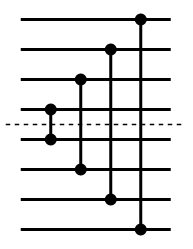
\includegraphics[width=0.47\columnwidth]{source/merger}
	\captionof*{figure}{Merger of width 8}
\end{minipage}%
\begin{minipage}{0.5\columnwidth}
	\centering
	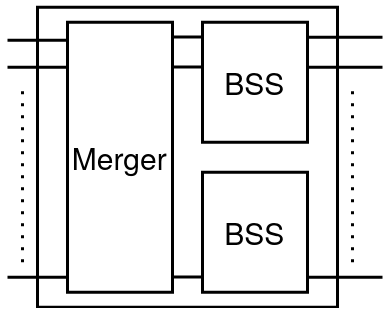
\includegraphics[width=0.75\columnwidth]{source/mn}
	\captionof*{figure}{Merging Network}
\end{minipage}
\vspace*{-1mm}

\textbf{Batcher}: A batcher sorting network of width $n$ consists of two batchers of width $n/2$ folowed by a merging network of width $n$. A batcher sorts an arbitrary sequence of width $n$. It has depth $\mathcal{O}(\log^2 n)$ and $\mathcal{O}(n \log^2 n)$ comparators. A batcher of width 1 is empty.

\vspace*{-1mm}
\begin{minipage}{\columnwidth}
	\centering
	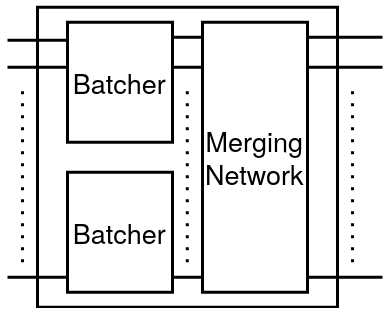
\includegraphics[width=0.4\columnwidth]{source/batcher}
	\captionof*{figure}{Batcher Sorting Network}
\end{minipage}

\begin{minipage}{\columnwidth}
	\centering
	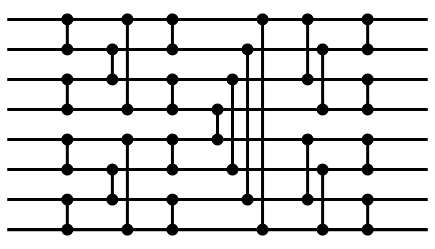
\includegraphics[width=0.58\columnwidth]{source/batcher8}
	\captionof*{figure}{Batcher Sorting Network of width 8}
\end{minipage}

\subsection{Counting Networks}

Counting networks are similar to sorting networks, but values arrive asynchronously.

\textbf{Definition 8.21} (Distributed Counting). A distributed counter is a variable
that is common to all processors in a system and that supports an atomic test-and-increment operation, which delivers the system’s counter value to
the requesting processor and increments it.

\textbf{Definition 8.22} (Balancer): A balancer is an asynchronous device which forwards messages that arrive on the left side to the wires on the right, the first to
the upper, the second to the lower, the third to the upper, and so on.

\textbf{Bitonic Counting Network}: Take a Batcher and replace all comparators by balancers. The resulting tokens passing the network exit the network in the order they arrived. This represents a very decentralized way of counting.

\textbf{Theorem 8.30} (Counting vs. Sorting): If a network is a counting network then it is also a sorting network, but not vice versa.

\section{Global Problems 1}

In global problems, it matters what happens far away in a graph. Coloring is a local problem since it only depends on neighbors. Learning the diamter $D$ of a graph on the other hand is a global problem.

\subsection{Diameter \& APSP}

Computing the diameter in a graph can be done by computing the \textbf{all-pairs-shortest-paths (APSP)} $\rightarrow$ max. APSP = diameter.

\textbf{Naive Diameter Construction}: All nodes compute their radius by synchronous flooding/echo. All nodes flood their radius on the constructed BFS tree. The maximum radius a node sees is the diameter. \textbf{Time}: $\mathcal{O}(D)$. Problem with this algorithm: nodes are involved in $n$ parallel flooding/echo operations $\rightarrow$ many big messages in one single step $\sim$ "cheating".

\textbf{CONGEST model}: In each round, each node can send one $B$ bit message to each of its neighbors. Each msg should have at most $B = \mathcal{O}(\log n)$ bits.

\textbf{Algorithm 9.3 (Compute APSP on G):} Computes diameter on graph $G$. First, a leader $l$ computes its BFS tree $BFS_l$. Then we send a pebble P to DFS-traverse tree $BFS_l$. Each time pebble P enters a node $v$ for the first time, P waits one time slot, and then starts a breadth first search (BFS) - using edges in G - from $v$ with the aim of computing the distances from $v$ to all other nodes. Since we start a $BFS_v$ from every node $v$, each node $u$ learns its distance to all these nodes $v$ during the according execution of $BFS_v$. There is no need for an echo-process at the end of $BFS_u$.\\
To get the diameter: at the end of the above alg, every node knows the distances to all other nodes. In particular, leader $l$ knows distance to farthest away leaf of $BFS_l$, let’s call that distance $D_l$. Now, if every node starts sending the maximal distance it
knows to its parent, starting from the leaves of $BFS_l$, $l$ knows the diameter after $D_l$ time. It can then broadcast it. \textbf{Time:} $\mathcal{O}(D) = \mathcal{O}(n)$.

\subsection{Lower Bound Graphs}

Lower bound graphs are a family of graphs $\mathcal{G}$ that are used to prove a lower bound on the number of rounds needed for some computation.

\textbf{Theorem 9.24:} Any distributed algorithm $\mathcal{A}$ that decides whether graph $G$ has diameter $D$ needs $\Omega(\frac{n}{\log n} + D)$ time.

This result can be shown using a $D=3$ LR-skeleton graph with inserted muscle edges and by applying results from communication complexity.


\subsection{Communication Complexity}

\textbf{Definition 9.11} (Communication complexity $CC(f)$):\\
In a two-party communication scenario, $CC(f) :=$ minimum number of bits the \textit{best} protocol needs to exchange at worst-case, such that the two parties can determine the value of a common function $f: \{0,1\}^k \times \{0,1\}^k \rightarrow \{0,1\}$, where one party has value $x$ and the other party has value $y$. 

\textbf{Matrix $M^f$}: For a given function $f$, define $2^k \times 2^k$ matrix $M^f$ representing $f$, i.e. $M_{x,y}^f := f(x,y)$.

\textbf{Monochromatic rectangle}: A set $R \subseteq \{0,1\}^k \times \{0,1\}^k$ is called a monochromatic rectangle if:

\vspace*{-1mm}
\begin{compactitem}
\item whenever $(x_1, y_1) \in R$ and $(x_2, y_2) \in R$ then $(x_1, y_2) \in R$.
\item there is a fixed $z$ s.t. $f(x,y,) = z, \forall (x,y) \in R$.
\end{compactitem}

\textbf{Fooling set:} A set $S \subset \{0,1\}^k \times \{0,1\}^k$ fools $f$ if there is a fixed $z$ such that

\vspace*{-1mm}
\begin{compactitem}
\item $f(x,y,) = z, \forall (x,y) \in S$
\item For any $(x_1, y_1) \neq (x_2, y_2) \in S$, the rectangle $\{x_1, x_2\} \times \{y_1, y_2\}$ is not monochromatic: either $f(x_1, y_2) \neq z$, $f(x_2, y_1) \neq z$, or both.
\end{compactitem}
\vspace*{-1mm}

\textbf{Lemma 9.18}: If $S$ is a fooling set for $f$, then $CC(f) = \Omega(\log |S|)$.

\textbf{Theorem 9.19}: $CC(EQ) = \Omega(k)$, where $EQ$ is the equality function on $\{0,1\}^k \times \{0,1\}^k$.

\textbf{Definition 9.20:} Denote the negation of a string $z$ by $\overline{z}$ and denote the concatenation of strings $x,y$ by $x \circ y$.

\textbf{Lemma 9.21:} Let $x,y$ be $k$-bit strings. Then $x \neq y$ if and only if there is an index $i \in [2k]$ s.t. the $i^{th}$ bit of $x \circ \overline{x}$ and the $i^{th}$ bit of $\overline{y} \circ y$ are both 0.

\textbf{DISJ}: $CC(DISJ) = \Omega(k)$, where $DISJ(x,y)$ is 0 if there is an index $i$ for which $x_i = y_i = 1$ (not disjoint), else 1.

\textbf{Parity}: $CC(PARITY) = 2$.

\textbf{Randomized evaluation of EQ}: Assume Alice and Bob both have access to the same random bit string $z \in \{0,1\}^k$. This allows them to check parity of $x \&\& z$ (Alice) and $y \&\& z$ (Bob), which has $CC(parity) = 2$.\\
Equivalent notion: Alice and Bob repeatedly check the some index $i$ of their bitstrings for equality, where $i$ is found through shared randomness.

\textbf{Lemma 9.26}: If $x \neq y$, the randomized evaluation of EQ discovers $x \neq y$ with probability at least $1/2$. $CC_{rand}(EQ) = \log k$. 

\textbf{Hamming distance:} $CC(HAM \geq d) = \Omega(d)$.

\section{Global Problems 2: MST}

Given a weighted tree $G = (V, E, \omega)$, where each edge $e$ has some weight $\omega(e)$. The MST is the spanning tree on $G$ that spans all nodes and the summed edge weights are minimal among all spanning trees.

The GHS algorithm (cf. Section 2) finds an MST in $\mathcal{O}(n \log n)$ rounds. In the worst case graph, one cannot be much faster than this (consider a $n$-node circle with small weights except for two huge weights $\rightarrow$ only one huge weight edge can be in the MST). At least $\Omega(n)$ rounds needed to compute MST on general graph.

\hl{\textbf{This section:} Focus on small diameter graphs $G$ with $D << n$.}


\textbf{Boruvka's MST algorithm:} Proceeds in $\log n$ phases. We have fragments. Initially, each node is its own fragment. Each node in a fragment proposes its minimum weight outgoing (MWO) edge. All MWO edges are added to forest and fragments are merged along MWO edges. Fragment leader finds MWO edge by flooding/echo $\rightarrow$ $\mathcal{O}(n)$. \textbf{Time:} $\mathcal{O}(n \log n)$.

\subsection{Improved Boruvka MST algorithm}
\hl{MST in $\mathcal{O}((D+\sqrt{n})\log n)$ rounds, $D << n$, CONGEST model.}

Again, $\log n$ phases. In each phase, we have fragments $S_i$. Each fragment has a leader $s_i \in S_i$. All nodes in a fragment know the leader and the number of nodes in the fragment (this information needs to be mainted using flooding/echo). The algorithm computes in each phase for each fragment its MWO edge in $\mathcal{O}(D + \sqrt{n})$ rounds.

Fragments are categorized into small and large fragments:

\vspace*{-2mm}
\begin{compactitem}
\item Small fragments: at most $\sqrt{n}$ nodes. MWO edges are found by using flooding inside the fragment: $\mathcal{O}(\sqrt{n})$ rounds.

\item Large fragments: at least $\sqrt{n}+1$ nodes. MWO edges are found by using flooding on the \textit{whole} graph $G$.
\end{compactitem}
\vspace*{-1mm}

Observation: There are at most $n/\sqrt{n} = \sqrt{n}$ large fragments. Flooding in large fragments on the whole graph can be done in $\mathcal{O}(D + \sqrt{n})$ rounds, using \textit{Pipelining}.

\hl{\textbf{Pipelining:}} Compute BFS tree in $\mathcal{O}(D)$ rounds. Round 1: leafs start sending MWO edges for $S_1$. Round 2: parents of leafs start sending, etc. Each node only forwards the min. edge per fragment. Since we have at most $\sqrt{n}$ large fragments, we have at most $\sqrt{n}$ pending msgs per node. After $\mathcal{O}(D)$ rounds, the root knows the MWO edge of fragment $S_1$. After $\sqrt{n}$ additional rounds, the root knows the MWO edges for all fragments. For flooding, the whole process can be done in reverse. \hl{\textbf{Time:} $\mathcal{O}(D + \sqrt{n})$.}

\textbf{Problem:} Arbitrarily merging fragments could result in long chains of fragments, which is problematic for information dissemination.\\
\textbf{Solution:} Break long chains using randomness. Each fragments tosses a coin (T/H). Merge arrows are \textit{only} accepted if they go from a tail (T) fragment to a head (H) fragment: T $\rightarrow$ H. The merged fragments then form a star.\\
Coin tosses are done in each new phase and the toss result is spread in the fragment using Pipelining in $\mathcal{O}(D + \sqrt{n})$ rounds.

\textbf{Analysis:} Why is it ok not to pick some MWO edges in some rounds? Claim: $\mathcal{O}(\log n)$ are still enough to merge all fragments w.h.p. A merge arrow is accepted with probability $\frac{1}{2} * \frac{1}{2} = \frac{1}{4}$. The $\mathcal{O}(\log n)$ round claim follows directly.


\section{Global Problems 3: Minimum Cut}

Minimum cut:

\vspace*{-1mm}
\begin{compactitem}
\item Unweighted graph: smallest number of edges whose removal disconnects the graph.
\item Weighted graph: smallest summation of edge weights s.t. the removal of the edges disconnects the graph.
\end{compactitem}

\textbf{Cut:} $cut_G\{S, V\backslash S\}$ denotes the set of edges that have one endpoint in $S$ and the other endpoint in $V\backslash S$. 

\textbf{Sparse certificates:} Given a graph $G = (V,E)$, we call a spanning subgraph $H = (V, E')$ a sparse certificate for $K'$-connectivity, if $H$ satisfies two conditions:

\begin{compactenum}
\item for each cut $(S, V\backslash S)$, we have cut size 
\vspace*{-2mm}
$$cut_H(S, V\backslash S) \geq min\{K', cut_G(S, V\backslash S)\}$$
\vspace*{-5mm}
\item $|E'| \leq n \cdot K'$ (not too many edges in $H$)
\end{compactenum}

Intuition behind 1.: $H$ tries to keep the cut size at least $K'$ for every cut \textit{unless} it cannot because $G$ itself doesn't have $K'$ edges in that cut, in which case $H$ keeps all edges of the cut in $G$.

Observation: Any graph of min-cut $K$ must have at least $\frac{nK}{2}$ edges. Sparse certificates try to reduce the \#edges towards this threshold while maintaining the min-cut size.

Example: any spanning tree $T$ on $G$ is a sparse certificate for $K' = 1$ on $G$.

\subsection{Computing a sparse certificate for any $K'$}

A simple local algorithm looks as follows: $K'$ iterations. In each iteration $i$, define $F_i$ to be a spanning maximal forest of $G \backslash \bigcup_{j=1}^{i-1} F_j$. At the end, the sparse certificate is $H = \bigcup_{j=1}^{K'} F_j$


\textbf{Distributed Implementation:} We want a distributed implementation of the above sparse certificate algorithm. In each phase $i$, compute forest $F_i$ in $\mathcal{O}((D+\sqrt{n})\log n)$, using the MST algorithm from section 10. Then, instead of removing edges $F_i$ from $G$, set their weight to $\infty$ (or practically to $n^2$).


\subsection{Approximation Algorithm for Minimum Cut}

The algorithm is a $(2+\epsilon)$ approximation of the minimum cut. Assume the min-cut size $K$ is known. \hl{\textbf{Time:} $\mathcal{O}(K(D+\sqrt{n})\log^3 n)$}

First, compute a sparse certificate $H$ for $K' = (1 + \epsilon/10)K$ connectivity. This can be done in $\mathcal{O}(K'(D+\sqrt{n})\log n)$ rounds. Now $H$ has \textit{all} the edges of the min-cut, so we can create auxiliary graph $H'$ where we \textit{"contract"} edges, meaning we merge them along edges of $G \backslash H$. $H'$ has all min-cut edges of $G$.
(In practice, edges are not contracted, instead nodes are just grouped into components).

After the contraction, there are two cases:

\vspace*{-1mm}
\begin{compactenum}
\item $H'$ has at least $\frac{n}{1 + \epsilon/10}$ components: we have many components but few edges ($|E'| \leq nK'$) thus the avg. degree is small\\ $\rightarrow$ at least one node has degree $\leq 2K(1 + \epsilon/10)^2 \leq (2+\epsilon)K$.
\vspace*{1mm}
\item $H'$ has less than $\frac{n}{1 + \epsilon/10}$ components: in this case, we can't directly find the min-cut. However, the number of components has decreased significantly. Thus, set $G = H'$ and run the algorithm again. After $\mathcal{O}(\log n)$ runs, the min. cut is found.
\end{compactenum}

We assumed $K$ is known. In practice we take guesses for $K$, for some guess results will match. For more details and distributed implementation, consider notes and script.

\subsection{Identifying Cut Edges}

On a graph $G = (V,E)$, we can \hl{identify all cut edges $e \in E$ in $\mathcal{O}(D)$ rounds}, in the \hl{CONGEST model} ($\mathcal{O}(\log n)$-bit msg).

\textbf{Algorithm:} 1) Compute a BFS tree $T$ on $G$ in $\mathcal{O}(D)$ rounds. 2) For each edge $e = (u,v) \in T$ find the LCA $w = LCA(u,v)$ and the height $h_w$ of the LCA. 3) For any node $v'$ let $l(v')$ be smallest height $h_w$ among all non-tree neighbors of $v'$ and let $l(v') = h_{v'}$ if $v'$ has no non-tree neighbors. 4) Let $min_v$ be the smallest value $l(v')$ among all descendants $v'$ of $v$. Now, every tree edge $e = (u,v)$, where $u$ is $v$'s parent, is a cut-edge iff $min_v > h_u$.


\section{All-to-all Communication}

\textbf{Congested Clique model:} $n$ nodes, synchronous round, assume network to be a \hl{\textbf{complete graph}}. Per round, each node $v$ can send $\mathcal{O}(\log n)$-bit msg along each edge, i.e. $\mathcal{O}(n \log n)$ bits in total.

W.l.o.g. we can assume IDs are 1,2,..., n.

\subsection{Routing in the all-to-all communication setting}

\textbf{Setup:} Have some \# of messages where each msg $m_i$ has a source node $s_i$ and a destination node $t_i$. Each node can be the source of many msgs, and many msgs can go to the same destination.

What instances of the routing problem can be solved in $\mathcal{O}(1)$ rounds?
\textbf{Necessary \& sufficient conditions:}

\begin{compactitem}
\item Each node can send at most $\mathcal{O}(n)$ messages.
\item Each node can receive at most $\mathcal{O}(n)$ messages.
\end{compactitem}

\textbf{Solving routing using edge coloring:} Given messages on graph $G$, create bipartite graph $H$ with $|V| = 2n$ nodes $V = \{l_1, l_2, ..., l_n, r_1, r_2, ..., r_n\}$. There is one edge $e = (l_i, r_j)$ for each message $m: i \rightarrow j$. Assume max. degree $\Delta$ in $H$.

We want to color the edges. $2\Delta - 1$ colors are definitely enough (each edge has at most $2\Delta - 2$ neighboring edges). Vizing: $\Delta+1$ colors are enough as well (non-trivial result).

Suppose that $\Delta \leq n/2$, so there is an edge coloring with $\leq n$ colors. Given an edge coloring on $H$, routing works as follows: For an edge $e = (l_i, r_j)$ (corresponding to message $m: i \rightarrow j$) of color $c(e) \in \{1,...,n\}$, route message $m$ over:

\vspace*{-4mm}
$$i \rightarrow c(e) \rightarrow j$$
\vspace*{-6mm}

\textbf{Claim:} Can send all messages in $2 = \mathcal{O}(1)$ rounds.\\
\textbf{Reason:} Consider any node $l_i$. Since we have a valid edge coloring in $H$, at most one edge $e = (l_i, r_j)$ has color $c(e)$ and thus at most one message is sent on edge $(l_i, c(e))$. The same argument holds of $r_j$ receiving a message. 

\textbf{Lemma 3.1:} $\mathcal{O}(\Delta)$ edge coloring in $H$ $\rightarrow$ $\mathcal{O}(\lceil \frac{\Delta}{n}\rceil )$ rounds. The condition $\Delta = \mathcal{O}(n)$ is thus sufficient for existence of a $\mathcal{O}(1)$ round routing algorithm.


\subsection{Solving the Routing Problem Distributedly}

Distributed \hl{$\mathcal{O}(1)$-round algorithm for cases where $\Delta = \mathcal{O}(\frac{n}{\log n})$, using randomness, with success probability $\geq 1 - 1/n^2$}.

Suppose $\Delta \leq \frac{n}{20\log n}$, i.e. each node is the source of at most $\frac{n}{20\log n}$ messages and the destination of at most $\frac{n}{20\log n}$ messages.

\textbf{Valiant's trick (random relay)}: make $5\log n$ copies of each msg and send each copy to an iid random relay. A msg fails if $\geq 2$ copies go through the edge it uses. We want that for each message, at least one copy succeeds w.h.p.\\

\textbf{Analysis:} 	Fix one msg $m: v \rightarrow u$, fix one of its $5\log n$ copies. Node $v$ has at most $\frac{n}{20\log n}$ messages and $5\log n$ copies for each, thus at most $\frac{n}{20\log n} \cdot 5\log n = \frac{n}{4}$ copies in total. Thus, at most $\frac{n}{4}$ intermediate nodes are blocked. Thus, the copy fails with prob. $\frac{1}{n} \cdot \frac{n}{4} = \frac{1}{4}$. Similarly, the copy fails with prob $\frac{1}{4}$ in the second step. By union bound, any copy fails with prob. at most $\frac{1}{2}$.\\
For each msg, the prob. of all copies failing is at most $(\frac{1}{2})^{5\log n} = n^{-5}$. Union bounding over all msgs, the prob. that at least one msg fails completely is $n^2 \cdot n^{-5} = n^{-3}$. Thus, w.h.p. $1 - \frac{1}{n^{3}}$ for each msg at least one copy arrives at its destination.

\section{Wireless Protocols}

In the wireless topologies studied in this lecture, the following assumption of the topology were made:

\begin{compactitem}
\item All $n$ nodes are in range of each other (clique).
\item Synchronous time slots known to all nodes. In each slot, every node can either transmit (tx) or receive (rcv).
\item In every time step at most 1 node can successfully transmit. When transmitting, nodes do not receive anything.
\item In every time step, nodes are either transmitting, receiving or sleeping. Therefore a transmitting node can’t know if his transmission was successful $\rightarrow$ ACKs required!
\end{compactitem}

\textbf{Collision detection CD}: Nodes can distinguish between 0, 1, $>$1 nodes transmitting in the same slot. Without CD, the cases 0, $>$1 nodes transmitting cannot be distinguished.

\textbf{Wireless leader election problem:} "How long does it take until a node can transmit successfully" $\rightarrow$ that node is then called the leader.

\textbf{Initialization}: Process of assigning IDs $1,..., n$ to $n$ nodes.

\textbf{Uniform:} $n$ is unknown. \textbf{Non-uniform:} $n$ is known to all nodes.

\subsection{Non-uniform leader election with CD}

\textbf{Algorithm 13.1:} Slotted Aloha\\
\hl{Every node sends his message with $\mathbb{P} = 1/n$} until successfully transmitted. With $X$ being an R.V. denoting the number of transmitting nodes per slot, we have $P[X=1] = n \cdot \frac{1}{n} \cdot (1-\frac{1}{n})^{n-1} \approx \frac{1}{e}$, thus the process takes $e$ slots in expectation.

\columnbreak

\textbf{Leader election with Slotted Aloha:} All nodes try to send \textit{wanna-be-leader} msgs including their ID, using slotted Aloha. Once a node $l$ successfully transmitted, all other nodes send a distributed acknowledgment (again using slotted Aloha) s.t. the $l$ knows that it is the leader. This terminates in (constant!) expected time $2e+1 = 6.42$. 

\textbf{Unslotted Aloha:} Time model with no synchronous slots. Messages interfere if they overlap partially. Thus, no msg can be sent in a slot of length $2*slot\_length$ (otherwise they'd overlap) $\rightarrow$ factor 2 penalty. The probability of successful transmission drops to $\frac{1}{2e}$ and the process finishes in expected time $2e$.

\subsection{Non-uniform Initialization}

\textbf{Theorem 13.3:} If the nodes know $n$, we can initialize them in $\mathcal{O}(n)$ rounds. This can be done by repeatedly doing leader election (see slotted Aloha). The new leader gets the next free ID and then leaves the process. $\mathbb{E}[rounds] = n \cdot e = \mathcal{O}(n)$.


\subsection{Uniform Initialization with CD}

\textbf{Algorithm 13.5:} In each slot, nodes are uniformly random split into two \textit{non-empty} groups. A slot is successful if no group is empty. If some node is alone in a group at some point, that node gets the next lowest free Id. Groups with more than one node are recursively split again.

\textbf{Theorem 13.6:} Algorithm 13.5 correctly initializes $n$ nodes in expected time $\mathcal{O}(n)$.


\subsection{Uniform Initialization without CD}

\textbf{Trick to run algs that require CD in topologies without CD:} 
Assume we have a special node $l$ (leader) and divide every time step in two. The msgs of the original algorithm are sent in \textit{both} steps. In the second step, $l$ sends a msg in addition to the regular msgs. Interference is “heard” as two consecutive unsuccessful transmissions, silence is “heard” as an unsuccessful followed by successful transmission. This trick works with all algorithms and results in an overhead of factor 2 in time and msg complexity.

More generally, a leader immediately brings CD to any protocol.

\vspace*{-2mm}
\begin{center}
\begin{tabular}{ccc}
	\toprule
	& $S$ transmit & $S \cup \{l\}$ transmit \\ 
	\toprule
	$|S| = 0$ & \xmark & \cellcolor{yellow}\cmark \\ 
	
	$|S| = 1 = \{l\}$ & \cellcolor{yellow}\cmark & \cellcolor{yellow}\cmark \\ 
	
	$|S| = 1 \neq \{l\}$ & \cellcolor{yellow}\cmark & \xmark \\ 
	
	$|S| \geq 2$ & \xmark & \xmark \\ 
	\bottomrule
\end{tabular} 
\end{center}


\textbf{Summary initialization:}
\vspace*{-2mm}
\begin{center}
\begin{tabular}{@{}ccc@{}}
	\hline 
	& uniform & non-uniform \\ 
	\hline 
	wo/ CD & Tree $\mathcal{O}(n)$ + leader & Aloha $\mathcal{O}(n)$ \\ 
	w/ CD & Tree $\mathcal{O}(n)$ & Aloha $\mathcal{O}(n)$ \\ 
	\hline 
\end{tabular} 
\end{center}

\subsection{Leader Election}

\subsubsection{Non-uniform Leader Election}

\textbf{Theorem 13.9:} Algorithm 13.1 elects a leader w.h.p. in $\mathcal{O}(\log n)$ time slots.\\
Proof: Probability of not finding a leader after $c\log n$ slots:

$(1 - 1/e)^{c\ln n} = (1 - 1/e)^{e\cdot c'\ln n} \leq \frac{1}{e^{c'\ln n}} = \frac{1}{n^{c'}}$

\subsubsection{Uniform Leader Election}

\textbf{Algorithm 13.10:} Uniform leader election, exponential backoff\\
Starting with $P_{send} = 1/2$, all nodes send \textit{wanna-be-leader} msgs. Probability $P_{send}$ is repeatedly halved. \hl{In phase $k$, all nodes transmit with probability $P_{send} = 1/2^k$ for $ck$ rounds (for some const. $c$)}. This is done until one node $v$ transmits alone, which then becomes leader. This algorithm essentially approximates $1/n$.

\textbf{Theorem 13.11:} By using \hl{Algorithm 13.10} it is possible to \hl{elect a leader w.h.p. in $\mathcal{O}(\log^2 n)$} time slots if $n$ is not known.


\textbf{Algorithm 13.12:} Fast Uniform leader election with CD\\
All nodes transmit with $P = 1/2$ \textit{wanna-be-leader} msgs. All nodes that do not transmit in a round leave the protocol if at least one node transmits. If a node transmits alone then he becomes the leader.

\textbf{Theorem 13.13:} With collision detection we can elect a leader using \hl{Algorithm 13.12 w.h.p. in $\mathcal{O}(\log n)$ time slots.}


\textbf{Algorithm 13.14:} Even faster uniform leader election\\
Algorithm runs in 3 phases, trying to find a good $\alpha$ to estimate $P= 1/2^\alpha \approxeq 1/n$. 
\begin{compactenum}
\item polyexponential backoff until silence (probabilities $1/2, 1/2^2, 1/2^4. 1/2^8, 1/2^16, ...$) $\mathcal{O}(\log \log n)$.
\item use a binary search on the interval found in phase 1. to improve the estimate. $\mathcal{O}(\log \log n)$.
\item use a probing to further improve the estimate. The algorithm stops after successful transmission of a single node, which then gets leader. $\mathcal{O}(\log \log n)$.
\end{compactenum}

\textbf{Theorem 13.23:} The Algorithm 13.14 elects a leader with probability of at least $1 - \frac{\log \log n}{\log n}$ in time $\mathcal{O}(\log \log n)$.


\subsection{Lower Bound}

\textbf{Theorem 13.24:} Any uniform protocol that elects a leader with probability of at least $1 - \frac{1}{2^t}$ must run for at least $t$ time slots.


\subsection{Uniform Asynchronous Wakeup}

\textbf{Theorem 13.25:} If nodes wake up in an arbitrary (worst-case) way, any algorithm may take $\Omega(n/ \log n)$ time slots until a single node can successfully transmit.

\vspace*{50mm}

\columnbreak

\section{Labeling Schemes}

We want to repeatedly query a huge graph (e.g. Facebook graph). A \textbf{labeling scheme} is an encoder $e$ and a decoder $d$. $e$ assigns to each node $v$ a label $e(v)$. $d$ answers some query based on the label of some nodes.

\textbf{Label size:} largest size (in bits) of a label assigned to a node.

\subsection{Adjacency}

\textbf{Theorem 14.1}: There exists a \hl{$2\log n$ labeling scheme for node adjacency in trees.} Proof: choose a root in the tree. Then, each node $u$'s label is $(u, p(u))$, where $u$ is $u$'s ID and $p(u)$ is the ID of $u$'s parent.

\textbf{Theorem 14.3:} There is a \hl{labeling scheme for adjacency in general graphs with label size of $\lfloor \frac{n}{2} \rfloor + \lceil \log n \rceil \approx \frac{n}{2}$}.\\
Proof: a node $u$ of ID $u$ has label

\vspace*{-2mm}
\begin{compactitem}
\item ID $u \in \{0, ..., n-1\}$
\item for $j = u+1 \mod n, ..., u+\lfloor \frac{n}{2} \rfloor \mod n$, one bit indicating adjacency to node $j$
\end{compactitem}

\textbf{Theorem 14.4:} Any labeling scheme for adjacency in general graphs has a label size of at least $\approx \frac{n}{2} \in \Omega(n)$ bits.


\subsection{Rooted Trees}

\textbf{Theorem 14.5:} There is a \hl{$2\log n$ labeling scheme for ancestry}, i.e. for two nodes $u, v$, find out if $u$ is an ancestor of $v$ in rooted tree $T$. Proof: DFS traverse $T$, which gives preorder index $l(u)$ for each node. A node $u$'s label then is $e(u) = (l(u), r(u))$, where $r(u)$ is the largest $l(v)$ index of any node $v$ in $u$'s subtree.

\textbf{Theorem 14.7} (Naive distance labeling in trees):\\
There is an $\mathcal{O}(n \log n)$ labeling scheme for distance in trees.

\textbf{Theorem 14.9} (Heavy-light decomposition): There is an \hl{$\mathcal{O}(\log^2 n)$ labeling scheme for distance in trees}.\\
Proof: For each node, partition child edges into heavy and light edges. Heavy edges lead to the child with the largest subtree. Labeling encodes the root-leaf path. Consecutive heavy edge paths are aggregated into the number of heavy edges taken (e.g. label (1,\textbf{4}, 1,1)).\\
One can further show that any labeling scheme for distance in trees needs to use labels of size at least $\Omega(\log^2 n)$.


\subsection{Road Networks}

Labeling schemes are used to quickly find shortest paths in road networks. In this section, we focus on distance only. 

\textbf{Encoder}: compute set of S of \textit{hub nodes} that lie on many shortest paths. Then at each node $u$, only store distances to hub nodes that appear on shortest paths originating or ending in $u$.

\textbf{Decoder}: Given two labels $e(u), e(v)$, let $H(u,v)$ denote the set of hub nodes that appear in both labels. The decoder then returns:
\vspace*{-1mm}
\begin{center}
$d(u,v) = \min\{dist(u,h) + dist(h,v) : h \in H(u,v)\}$.
\end{center}


\textbf{Algorithm 14.10} (Naive-Hub-Labeling(G)):\\
Iteratively find the hub $h$ that appears on most shortest paths $p \in P$, add $h$ to label of all endpoints of paths $p$ and remove paths $p$ from set of all $n^2$ shortest paths $P$. Repeat until $P = \emptyset$.

\textbf{Shortest path cover:} Node set $S_i$ is a shortest path cover if $S_i$ contains a node on every shortest path of length in $[2^{i-1}, 2^i]$.

\textbf{Algorithm 14.11} (Hub-Labeling(G)):\\
Encoder constructs shortest path covers. At node $v$ only the hub nodes in $S_i$ that are within the ball of radius $2^i$ around $v$ (denoted by $B(v, 2^i)$) are stored. For all $v \in V$, we then have $F_i(v) := S_i \cap B(v, 2^i)$ and $F(v) := F_1(v) \cup F_2(v) \cup ...$. The label of $v$ consists of the nodes in $F(v)$, with their distance to $v$.

\textbf{Highway dimension:} The parameter $h := max_{i,v} F_i(v)$ is the so called highway dimension of $G$.

\vspace*{150mm}

\columnbreak

\section{Appendix}

\subsection{General}

\textbf{Definition 13.8 (With High Probability)}: Some probabilistic event is said to occur with high probability (w.h.p.), if it happens with a probability $p \geq 1 - \frac{1}{n^c}$, where $c$ is a constant. The constant $c$ may be chosen arbitrarily, but it is considered constant with respect to Big-O notation.


\subsection{Proving concepts}

\begin{compactitem}
\item In anonymous symmetrical topologies one can often argue that all nodes are always in the same state, since inputs are equal and the topology looks the same from every nodes point of view.

\item Argue with speed of information in big topologies: “..node x can’t know shit about node y in the given time t since they are more than t apart..”
\item To reduce a bound using number of edges m to a bound using
number of nodes n, assume clique because it has maximum $m = \frac{n(n-1)}{2}$.

\item Proving w.h.p.: Consider number of rounds $c*f(n)$ to prove round complexity of an $f(n)$ algorithm, for some (large) constant $c$. Then consider failure probability $P[fail]$ and calculate the probability that after $c*f(n)$ rounds, the algorithm is not finished yet. Usually, the w.h.p. result follows directly.
\end{compactitem}

\subsection{Tricks \& Gotchas}

\begin{compactitem}
\item To start an algorithm at leaves of a tree: Upon receiving all messages of your children do ...
\item Make sure to cover $n = 1, 2$ in custom algorithms, if $n \geq 3$ or
something like this is not given!
\item Asynchronous model: Nodes have to wake up! Algorithm starts when first node wakes up
\item $\mathcal{O}(D + k)$ round complexity: often pipelining of $k$ values.
\item \hl{Often used concept: color graph and use color for scheduling.}
\end{compactitem}

\subsection{Big-O and Friends}

\begin{compactitem}
\item $f \in \mathcal{O}(g) \Leftrightarrow f \leq g \Leftrightarrow \lim\limits_{n\rightarrow \infty} \frac{f(n)}{g(n)} < \infty$
\item $f \in o(g) \Leftrightarrow f < g \Leftrightarrow \lim\limits_{n\rightarrow \infty} \frac{f(n)}{g(n)} < 0$
\item $f \in \Omega(g) \Leftrightarrow f \geq g \Leftrightarrow \lim\limits_{n\rightarrow \infty} \frac{f(n)}{g(n)} > 0$
\item $f \in \omega(g) \Leftrightarrow f > g \Leftrightarrow \lim\limits_{n\rightarrow \infty} \frac{f(n)}{g(n)} = \infty$
\item $f \in \Theta(g) \Leftrightarrow f = g \Leftrightarrow f \in \mathcal{O}(g) \cap \Omega(g)$
\end{compactitem}

Note: $o(1)$ are functions that tend to 0 as $x$ tends to infinity.


\subsection{Time complexity}

\begin{compactitem}
\item $\mathcal{O}(\log_2(t))$ $\Leftrightarrow$ In every time step "half the problem" is solved.
\item $\mathcal{O}(t)$ $\Leftrightarrow$ All nodes have to do something sequentially.
\item $\mathcal{O}(t^2)$ $\Leftrightarrow$ One node after another sends something to all nodes.
\end{compactitem}

$$n\log n > n > \frac{n}{\log n} > \sqrt{n} > \log^2 n > \log n > \log\log n$$


\subsection{Useful formulas}

\textbf{Geometric series:} $$\sum_{k=0}^{\infty} q^k = \frac{1}{1-q} \qquad \text{ if } |q| < 1$$

\textbf{Gauss sum:} $$\sum_{i=1}^{n} i = \frac{n(n+1)}{2}$$

\textbf{Union bound:} For a countable set of events $E_1, E_2, E_3, ...$ we have $$Pr\big[\bigcup_{i} E_i\big] \leq \sum_{i} Pr[E_i]$$

\textbf{Markov’s inequality:} If $X$ is any random variable and $a > 0$, then $$Pr[|X| \geq a] \leq \frac{E[X]}{a}$$

\textbf{Chernoff bound:} Let $Y_1, ..., Y_n$ be independent Bernoulli random variables and let $Y := \sum_{i} Y_i$.\\
For any $0 \leq \delta \leq 1$ it holds
\vspace*{-3mm}
$$PR[Y \leq (1 - \delta)E[Y]] \leq e^{-\frac{\delta^2}{2}E[Y]}$$
and for $\delta \geq 0$ 
\vspace*{-3mm}
$$PR[Y \geq (1 + \delta)E[Y]] \leq e^{-\frac{min(\delta, \delta^2)}{2}E[Y]}$$
\vspace*{-5mm}
$$PR[Y \geq (1 + \delta)E[Y]] \leq e^{-\frac{\delta^2}{2+\delta}E[Y]}$$

\textbf{Theorem 13.29:} We have $$e^t \big( 1-\frac{t^2}{n} \big) \leq \big( 1 + \frac{t}{n} \big)^n \leq e^t$$

\textbf{Theorem 13.30:} For all p, k such that $0 < p < 1$ and $k \geq 1$ we have $$1 - p \leq (1 - p/k)^k$$

\textbf{Useful inequality:} $$2^{-x} \geq e^{-x} \geq 1-x \geq 4^{-x}\qquad \text{ for } x \leq 1/2$$

\textbf{Triangle inequality} (useful for node distances) $$d(u,w) \leq d(u,v) + d(v,w)$$

\textbf{Lemma 7.13}: For $\alpha > 1$, $1 + \log(\alpha - 1)/2 \leq \log \alpha$.

\columnbreak

\subsection{Graphs}

If you swap edges of vertices of a graph, you get a \textbf{line graph}. It holds that \hl{$\Delta_{\text{line graph}} \leq 2(\Delta_{\text{orig. graph}}-1)$} since an edge is adjacent to at most $\Delta_{\text{orig. graph}}-1$ other edges at both node endpoints.

\begin{center}
\renewcommand{\arraystretch}{1.2}
\begin{tabular}{@{}p{22mm}p{50mm}@{}}
	\hline 
	Graph & Properties \\ 
	\hline
	Clique (complete graph $K_n$) & $d(v) = n-1, \forall v \in V$, $m = \binom{n}{2} = \frac{n(n-1)}{2}$ edges, $\chi(K_n) = n$ \\ 
	 
	Bipartite graph & $\chi \leq 2 \Leftrightarrow$ no odd cycle \\ 
	 
	Tree & $m = n-1$ edges, any simple path between $u,v$ is the shortest path \\ 
	 
	Hypercube of dimension $d$ & $n = 2^d$ vertices, are bipartite \\ 
	\hline 
\end{tabular} 
\end{center}

\subsubsection{Planar Graphs}

\textbf{Definition:} A graph $G$ is planar if it can be represented by a drawing in the plane so that no edges cross.

\textbf{Theorem:} For a simple, connected, planar graph with $n$ vertices and $m$ edges and $f$ faces, the following simple conditions hold for $n \geq 3$:

\begin{compactitem}
\item $m \leq 3n - 6$
\item If there are no cycles of length 3, then $m \leq 2v -4$
\item $f \leq 2v - 4$
\end{compactitem} 

\textbf{Theorem:} $K_5$ is not planar.

\textbf{Theorem:} If $G$ is planar, $G$ has maximum degree $\Delta = 5$.

\textbf{Theorem} (Five Color Theorem): Every planar graph can be colored with 5 colors.






\subsection{Algorithm approaches}

\begin{compactitem}
\item Unbounded msg size, $\mathcal{O}(poly(\log n))$ complexity: $(C,D)$ network decomposition.

\item $\mathcal{O}((D+f(n))g(n))$: pipelining

\item $\mathcal{O}(f(n)\cdot \log n)$: round based algorithm with some multiplicative increase/ decrease
	
\item Matching/ maximal matching: edge coloring

\item Independent/ dominating set: vertex coloring

\item With high probability $1-1/n^c$: uniform at random selection, failure probability, Chernoff bound

\item If all nodes at distance $d$ from node $v$ need to be processed independently, create an auxiliary graph $G^d$ where you add edges between all nodes that have distance $d$ from each other.
\end{compactitem}


\subsection{Useful facts}

\begin{compactitem}
\item Graphs with diameter $D = 1$ are fully connected, i.e. each node has equal degree $d(v) = n-1$.

\item Color a hypercube: sum up number of 1s in Id and 2-color based on the $\mod 2$ of the number of 1s.
\end{compactitem}

\columnbreak

\subsection{Log Rules}

\begin{compactitem}
\item $\log_b(b^y) = y$

\item $\log_b(x \cdot y) = \log_b(x) + \log_b(y)$

\item $\log_b(x / y) = \log_b(x) - \log_b(y)$

\item $\log_b(c) = 1 / \log_c(b)$

\item $\log_b(x) = \log_c(x) / \log_c(b)$
\end{compactitem}

\subsection{Derivative Rules}

\begin{compactitem}
	\item $(af)' = af'$
	
	\item $(f+g)' = f' + g'$
	
	\item $h = f\cdot g, h' = f'\cdot g + f \cdot g'$
	
	\item $h'(x) = (f(g(x)))' = f'(g(x))\cdot g'(x)$
	
	\item $(\frac{f}{g})' = \frac{f'g - g'f}{g^2}$
\end{compactitem}





	
\end{multicols*}

\setcounter{secnumdepth}{2}
\end{document}